\chapter{Cryptography Introduction}
\section{Cryptosystem}
    \paragraph{Definizione} Un \textbf{cryptosystem} è una tupla di 5 elementi (E,D,M,K,C):
    \begin{description}
        \item[E] è un \textit{algoritmo di cifratura}
        \item[D] è un \textit{algoritmo di de-cifratura}
        \item[M] è un insieme di \textit{messaggi in chiaro}
        \item[K] è un insieme di \textit{chiavi}
        \item[C] è un insieme di \textit{messaggi cifrati}
    \end{description}
    In modo astratto i punti \textbf{E} e \textbf{D} possono essere espresse come funzioni:
    $$
        \begin{aligned}
            E: M \times K \rightarrow C \\
            D: C \times K \rightarrow M
        \end{aligned}
        \qquad D(E(m,k),k) = m
    $$
    Nella criptografia base ogni chiave $ k \in K $ può essere usata per cifrare e de-cifrare i messaggi, nella criptografia simmetrica la chiave è la stessa per entrambi i processi, mentre nella criptografia asimmetrica le chiavi sono diverse.
    \paragraph{Quali componenti sono pubbliche?} Solitamente non abbiamo necessità di mantenere segrete le funzioni \texttt{E} e \texttt{D} o il messaggio cifrato \texttt{C}, quello che davvero deve essere segreto è la chiave \texttt{K}. Il motivo per il quale le funzioni non devono essere segrete è che il sistema deve essere pubblico e quindi tramite processi di \textit{reverse engineering} è possibile ricavare le funzioni (es: il sistema di cifratura di un DVD è stato ricavato tramite \textit{reverse engineering} dopo solo due giorni).
    \subsection{Why Cryptography?}
        \paragraph{Sicurezza} La crittografia è usata nei \hyperref[subsec:securityMechanism]{\textbf{meccanismi di sicurezza}} per garantire \hyperref[subPar:confidentiality]{\textbf{confidenzialità}} nascondendo il contenuto dei messaggi, \hyperref[subPar:integrity]{\textbf{integrità}} provvedendo al controllo di integrità tramite funzioni di \textbf{hash} e \textbf{la verifica dell'origine} dei dati tramite firme digitali verificabili da una fonte autorevole.
    \subsection{Cryptography on rented servers}
        \paragraph{Problema} Se si usa un server di terze parti per conservare dati, ad esempio su un database, è possibile che il proprietario del server possa accedere ai dati in chiaro. Per evitare ciò si può cifrare i dati prima di inviarli al server, in modo che il proprietario non possa leggerli, ciò comporta però un aumento del carico computazionale lato client in quanto tutti i dati prima di essere letti devono essere de-cifrati, per questo esistono meccanismi di ricerca su dati cifrati che permettono di effettuare ricerche su dati cifrati senza de-cifrarli, una volta trovati i dati desiderati si de-cifrano solo quelli.
    \subsection{Come definiamo "Computazionalmente sicuro" nelle comunicazioni}
        \paragraph{Definzizione} Definiamo un sistema di comunicazione \textbf{Computazionalmente sicuro} quando la decifrazione di un messaggio cifrato senza conoscere la chiave è molto difficile, o addirittura impossibile, e richiede molto tempo e risorse computazionali.
        \paragraph{$E(k,P)=C$} Calcolare $C$ da $P$ deve essere difficile senza $k$, inoltre calcolare $C$ da $P$ sapendo $k$ deve essere facile.
        \paragraph{$D(k,C)=P$} Calcolare $P$ da $C$ deve essere facile sapendo $k$, ma deve essere difficile senza $k$.
        \paragraph{Trapdoor - funzione a senso unico} Una \textbf{trapdoor} è una funzione a senso unico che richiede una ulteriore informazione. Ed una \textbf{funzione a senso unico} è descritta come una funzione che è facile da calcolare in una direzione, ma molto più difficile nell'altra.  
    \subsection{Hash v/s Encryption}
        \paragraph{Quando l'una e quando l'altra} Usiamo funzioni di hash quando non abbiamo bisogno di accedere all'informazione originale, ma solo di verificare l'integrità dei dati. Ricordiamo che le funzioni di \textbf{hash} per definizione sono \textbf{one-way} e \textbf{deterministiche}, quindi non possiamo de-cifrarle e non necessitiamo di una chiave per cifrare i dati. \newline
        D'altro canto usiamo la cifratura quando i dati che vogliamo proteggere devono poter essere letti e ne vogliamo preservare la \textbf{confidenzialità}, bisogna prima concordare una \textbf{chiave} in maniera sicura, poi calcolare il \textbf{messaggio cifrato} con suddetta chiave e infine inviare il messaggio cifrato, il destinatario potrà de-cifrare il messaggio con la chiave concordata. In questo modo proteggiamo la \textbf{confidenzialità} e la \textbf{riservatezza} dei dati ma non la loro \textbf{integrità}.
    \subsection{La Criptografia non è la soluzione a tutti i problemi}
        \paragraph{Perchè?} La crittografia non è la soluzione a tutti i problemi di sicurezza, in quanto comunque è sensibile a delle chiavi conservate su supporti digitali, i quali devono proteggere questa informazione. Inoltre da sola la crittografia non è mai usata come soluzione a problemi di sicurezza, ma sempre in combinazione con altri meccanismi di sicurezza.
\section{Types of cryptography - Tipologie di criptografia}
    \subsection{Cifrari di sostituzione}
        \paragraph{In breve} I \textbf{cifrari di sostituzione} sono cifrari che sostituiscono un simbolo del \textit{dizionario} con un altro simbolo. In questo contesto la \textit{chiave} è la \textit{sostituzione} dei simboli.
        \paragraph{In lungo}
            I \textbf{cifrari di sostituzione} sono dei \textbf{metodi di criptazione} per i quali ogni simbolo del \textbf{messaggio in chiaro} è rimpiazzato nel \textbf{messaggio cifrato} rispetto ad un prefissato sistema. I "simboli" possono essere lettere, coppie di lettere, triple di lettere, o anche una combinazione di questi, e anche altro. Il ricevente decifra il testo svolgendo le sostituzioni inverse.
        \subsubsection{Cifrario di cesare}
            Il \textbf{cifrario di Cesare} è un cifrario di sostituzione in cui il \textbf{dizionario} del testo in chiaro è spostato di un numero fisso di posizioni nell'alfabeto. Per decifrare il testo cifrato si sposta indietro dello stesso numero di posizioni.\newline
            Questo tipo di sistema viene anche chiamato: \textbf{rotazione di $k$ posizioni}, in quanto il dizionario viene ruotato di $k$ posizioni.
            \paragraph{Problemi e proprietà} Il cifrario descritto è il più semplice tra tutti come decodifica in quanto esistono solo $25$ chiavi e con un semplice attacco di \textbf{brute force}. Inoltre se non si vuole usare un attacco di \textbf{brute force} si può comunque cercare di trovare lettere comuni del messaggio cifrato e provare a ricondurle a lettere comuni dell'alfabeto.
            \begin{figure}[H]
                \centering
                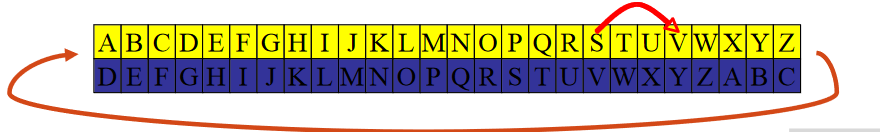
\includegraphics[width=0.9\textwidth]{03/cifrarioCesare.png}
                \caption{Esempio di cifrario di Cesare spostato di 3 posizioni}
            \end{figure}
        \subsubsection{Cifrario di Vigenère}
            Il \textbf{cifrario di Vigenère} è un cifrario che prevede l'uso di una "parola chiave", se necessario ripetuta per la lunghezza del messaggio, per poi calcolare la "somma" dei valori di ogni lettera del messaggio con la corrispondente lettera della parola chiave (prendendo poi il resto della divisione per 26). Quindi assegnando ad ogni lettera un numero da 0 a 25, si somma il numero della lettera del messaggio con il numero della lettera della parola chiave, si prende il resto della divisione per 26 e si assegna alla lettera corrispondente il numero ottenuto.
            \begin{figure}[H]
                \centering
                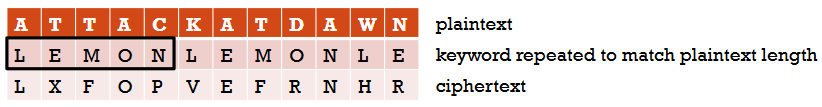
\includegraphics[width=0.9\textwidth]{03/cifrario2.png}
                \caption{Esempio di cifrario di Vigenère chiave "lemon"}
            \end{figure}
            Per decifrare il messaggio cifrato si sottrae il numero della lettera della parola chiave al numero della lettera del messaggio e si prende il resto della divisione per 26.
            \paragraph{Vantaggi} Questo cifrario è molto più sicuro rispetto a quello di cesare in quanto come mostrato nell'esempio la lettera "A" viene codificata in quattro lettere diverse e la lettera "T" che è presente tre volte viene cifrata in due lettere corrispondenti. In quanto la parola chiave ha lunghezza "l" allora dimensione della chiave è $l^{26}$. Inoltre se la chiave è della stessa lunghezza del messaggio allora il cifrario di Vigenère è equivalente a un cifrario di sostituzione casuale il che rende impossibile la decifrazione, però ciò comporta ad una ulteriore difficoltà per il mittente e il destinatario nel concordare una chiave.
    \subsection{Cifrari di trasposizione}
        \paragraph{In breve} I \textbf{cifrari di trasposizione} sono cifrari che permutano i simboli del messaggio in chiaro. In questo contesto la \textit{chiave} è la \textit{permutazione} dei simboli.
        \paragraph{In lungo} I \textbf{cifrari di trasposizione} sono dei \textbf{metodi di criptazione} per i quali i simboli del \textbf{messaggio in chiaro} sono permutati in un certo modo per ottenere il \textbf{messaggio cifrato}. Il ricevente decifra il testo svolgendo le permutazioni inverse.
        \subsubsection{Cifrario di trasposizione per colonne}
            Il \textbf{cifrario di trasposizione per colonne} è un cifrario che permuta i simboli del messaggio in chiaro per colonne, in modo che il messaggio cifrato sia una matrice di colonne.
            \begin{figure}[H]
                \centering
                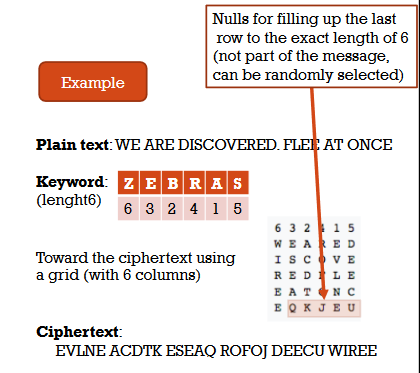
\includegraphics[width=0.5\textwidth]{03/cifrario3.png}
                \caption{Esempio di cifrario di trasposizione per colonne}
            \end{figure}
            Per decifrare il messaggio cifrato si riordinano le colonne in base alla chiave.
    \subsection{Criptografia Simmetrica}
        Come detto in precedenza la \textbf{criptografia simmetrica} prevede la stessa \textbf{chiave} per cifrare e de-cifrare i messaggi. La gestione di chi possiede le chiavi determina chi può accedere ai dati.
        \paragraph{Tipi} Esistono nella \textit{criptografia moderna} due tipi ci crittografia simmetrica:
        \begin{description}
            \item[Cifrari a flusso] I \textbf{cifrari a flusso} cifrano una "breve" porzione di un blocco di dati alla volta con una chiave che varia nel tempo. Questa tipologia si base su un \textbf{generatore di chiavi}, la cifratura è relativamente semplice (es. \texttt{XOR}) e molto spesso viene usato un bit per blocco.
            \item[Cifrari a blocchi] I \textbf{cifrari a blocchi} cifrano un blocco di dati "lungo" alla volta con una chiave fissa. Questa tipologia è più complessa e richiede uan funzione di cifratura e una di de-cifratura. Solitamente si usano blocchi di 64/128 bit.  
        \end{description}
        \subsubsection{Cifrari a flusso}
            I cifrari a flusso operano su un flusso di \textit{testo in chiaro} e producono un flusso di \textit{testo cifrato}. Lo stesso testo se ripetuto può essere cifrato in modo diverso in base al tempo nel quale è stato cifrato. I circuiti sono molto semplici e progettati per essere molto veloci.
            \begin{figure}[H]
                \centering
                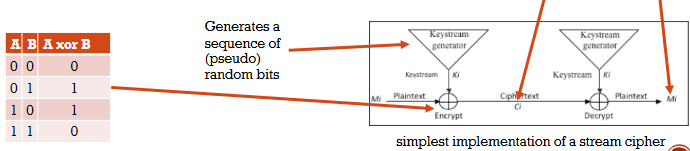
\includegraphics[width=0.9\textwidth]{03/cifrarioFlusso.png}
                \caption{Esempio di circuito di cifratura a flusso}
            \end{figure}
            \paragraph{Dove si usano} I cifrari a flusso sono usati in applicazioni in cui la velocità è fondamentale, come ad esempio nelle comunicazioni via radio o nella comunicazione in tempo reale.
        \subsubsection{Cifrari a blocchi}
            Nei \textbf{cifrari a blocchi} vene trattato una sezione di \textit{testo in chiaro} come una cosa unica per produrre un \textit{testo cifrato} di egual lunghezza. La dimensione tipica di questa sezione è solitamente tra $64$ e $128$ bit. Un messaggio $M$ più lungo di $n$ bit viene diviso in blocchi di $n$ bit e ogni blocco ($M_1, M_2, \dots, M_i$) viene cifrato separatamente con la stessa chiave $k$.
            \paragraph{Esempi} Alcuni esempi di cifrari a blocchi sono:
            \begin{description}
                \item[DES] \textbf{Data Encryption Standard} è un cifrario a blocchi che opera su blocchi di $64$ bit.
                \item[AES] \textbf{Advanced Encryption Standard} è un cifrario a blocchi che opera su blocchi di $128$ bit e utilizza chiavi di $128$, $192$ o $256$ bit.
            \end{description}
            \paragraph{DES}
                Il \textbf{Data Encryption Standard} è un cifrario a blocchi che opera su blocchi di $64$ bit che venne progettato da \texttt{IBM} negli anni '70. Il cifrario è basato su una rete di sostituzione e trasposizione, e utilizza una chiave di $56$ bit. Il DES è stato il cifrario più usato fino al 2000 (anche da ANS\footnote{American National Standard X3.92} e in tre F.I.P.S.\footnote{Federal Information Processing Standards}), fino al 2005 quando è stato definitivamente dichiarato insicuro.
            \paragraph{Feistel (1973)}
                Il cifrario DES è basato su una struttura di \textbf{Feistel}, la quale prevede che il testo in chiaro venga diviso in due parti uguali, la prima passa attraverso una funzione di cifratura insieme ad una chiave, il risultato viene messo in \textbf{XOR} con la seconda parte del testo in chiaro, il risultato viene poi scambiato con la prima parte e il processo viene ripetuto per $16$ volte con $16$ chiavi diverse (o una chiave divisa in $16$ parti). La decodifica avviene tramite lo stesso processo ma con le chiavi e le parti invertite.
                \subparagraph{Vantaggi e svantaggi} Primo vantaggio di questo algoritmo è lo stesso meccanismo di cifratura e de-cifratura oltre alla semplicità, questo rende le componenti hardware molto più semplici e meno costose in quanto non necessitano di componenti diverse per cifrare e de-cifrare. 
            \paragraph{AES} \label{par:AES}
                L'\textbf{Advanced Encryption Standard} è un cifrario a blocchi sviluppato come successore del \texttt{DES} dal dicembre 2001. L'\texttt{AES} usa una chiave simmetrica in uno schema chiamato \textbf{Rijndael}.\newline
                Il processo di cifratura è basato su una serie di tabelle che contengono le operazioni da eseguire e di operazioni \texttt{XOR} che sono molto veloci e semplici conoscendo la chiave, l'operazione di de-cifratura è la stessa ma con le tabelle invertite. Tuttavia anche se il processo è lo stesso bisogna costruire hardware e software diversi per cifrare e de-cifrare.
    \subsection{Criptografia Asimmetrica}
        La \textbf{criptografia asimmetrica} anche chiamata \textbf{\textit{Crittografia a chiave pubblica}} \textbf{\texttt{PKC}} prevede l'uso di due chiavi diverse, una per cifrare e una per de-cifrare. Questo sistema viene usato per avere una comunicazione sicura tra due parti in un contesto non sicuro.
        \paragraph{One way function} Le \textbf{funzioni one way} sono funzioni matematiche che costituiscono la base della crittografia asimmetrica, queste funzioni sono facili da calcolare in una direzione ma molto difficili nell'altra. Nella crittografia asimmetrica tuttavia usiamo funzioni \textit{one-way} che contengono una così detta \textit{trapdoor} o \textit{backdoor} che permette di invertire la funzione in modo semplice se si conosce un certo parametro.
        \subparagraph{Caso dell'\texttt{RSA}}
            Nell'\texttt{RSA} viene usata una funzione matematica che è facile da calcolare in una direzione ma molto difficile nell'altra, ovvero la \textbf{fattorizzazione di numeri primi}.
        \paragraph{Le chiavi} Le due chiavi usate nella crittografia asimmetrica sono due, una per cifrare e una per de-cifrare, la chiave pubblica è usata per cifrare i messaggi e la chiave privata è usata per de-cifrarli. La chiave pubblica è distribuita a tutti. Queste chiavi sono diverse ma corelate matematicamente anche se la conoscenza di una non permette la conoscenza dell'altra.
        \subsubsection{\texttt{RSA} - \textit{(Rivest, Shamir, Adleman)}}
            \label{subsubsec:RSA}
            L'\texttt{RSA} è un algoritmo di crittografia asimmetrica più usato al mondo, è basato sulla difficoltà di fattorizzare numeri primi molto grandi. L'algoritmo è stato inventato nel 1977 da \texttt{Ron Rivest}, \texttt{Adi Shamir} e \texttt{Leonard Adleman}. Oggi è il sistema di crittografia più usato al mondo e viene usato per scambio di chiavi, firme digitali e per la crittografia di dati.
            \paragraph{Funzionamento} Si prendono due numeri $ p $ e $ q $ entrambi primi molto grandi \footnote{generatore di numeri casuali e controllo che questi siano primi}, poi si calcola il prodotto $N=p\cdot q$ questo sarà il \textbf{modulo}. Ora si prende un qualsiasi numero $ e $ tale che questo sia primo rispetto a $ (p-1)(q-1) $, con questo troviamo $ d $ definito come l'inverso del modulo $ e $ come $ d\cdot e = 1 \mod (p-1)(q-1) $. La chiave pubblica sarà $ (N,e) $ e la chiave privata sarà $ (N,d) $. Assumendo quindi che $ M $ con $ 0 < M < N $ sia il messaggio da cifrare, il messaggio cifrato sarà $ C = M^e \mod N $ e il messaggio de-cifrato sarà $ M = C^d \mod N $. Notare come $ C^d \mod N = (M^e \mod N)^d \mod N = M^{ed} \mod N = M $.
            \subparagraph{Attacchi} In quanto $ N $ e $ e $ sono pubblici se un attaccante riesce a fattorizzare $ N $ allora può usarlo per calcolarsi $ d $ e quindi de-cifrare i messaggi in quanto $ e\cdot d = 1 \mod (p-1)(q-1) $. Per questo motivo è importante che $ N $ sia molto grande e che $ p $ e $ q $ siano molto grandi. 
            \paragraph{Un problema recente con \texttt{RSA}} Recentemente è stato scoperto un problema relativo alla generazioni di chiavi \texttt{RSA} infatti una libreria software usata nelle \textit{smartcard}, \textit{security tokens} e \textit{trusted platform modules} per generare chiavi \texttt{RSA} presentava una vulnerabilità: la libreria non generava in modo casuale le chiavi ma usava un generatore di numeri pseudo-casuali che permetteva di conoscere la chiave privata conoscendo la chiave pubblica. Questo problema è stato riscontrato in molti dispositivi che sono stati prodotti con questa libreria, questi dispositivi sono stati ritirati dal mercato e sostituiti.
            \paragraph{Integrità con \texttt{RSA}}
                Per verificare l'integrità di un messaggio si può usare la crittografia \texttt{RSA} a proprio vantaggio. Prendiamo un messaggio, ce ne calcoliamo l'\textit{hash} tramite una funzione di \textit{hashing}, ora grazie alla chiave privata il mittente cifra il \textit{digest} ottenuto e invia messaggio e \textit{digest} cifrato al destinatario. Il destinatario de-cifra il \textit{digest} grazie alla chiave pubblica del mittente e confronta e ri-calcola l'\textit{hash} del messaggio, se i due \textit{digest} coincidono allora il messaggio è integro, altrimenti se non coincidono il messaggio è stato alterato (o il messaggio o il \textit{digest}).
            \paragraph{Problemi dell'\texttt{RSA}} In generale l'unico reale problema dell'\texttt{RSA} è la lentezza, infatti la generazione delle chiavi è molto lenta e la cifratura e de-cifratura sono molto lente, per questo motivo l'\texttt{RSA} viene usato solo per scambiare chiavi simmetriche che verranno poi usate per cifrare i messaggi. In questo modo si combina la sicurezza dell'\texttt{RSA} con la velocità dei cifrari simmetrici.
                \subparagraph{\textit{store now decrypt later}} Peccato che in questo modo si è esposti ad attacchi del genere \textit{store now decrypt later} ovvero se un attaccante riesce a intercettare tutti i messaggi compreso lo scambio di una chiave allora quando sarà riuscito a de-cifrare il messaggio con la chiave simmetrica potrà de-cifrare tutti i messaggi scambiati.
                \subparagraph{Pubblicazione della chiave privata} Un altro modo per attaccare un sistema crittografico basato su \texttt{RSA} è quello che per un qualunque motivo la chiave privata venga pubblicata, in questo caso l'attaccante può de-cifrare tutti i messaggi cifrati con la chiave pubblica, e se la chiave pubblica è usata per firmare i messaggi allora l'attaccante può falsificare i messaggi. In questa situazione la coppia di chiavi deve essere revocata e sostituita con una nuova coppia.

            \subsubsection{\texttt{DH} - \textit{Diffie-Hellman}}
                La cifratura \texttt{DH}è un algoritmo crittografico che permette a due parti di scambiarsi una chiave senza che questa venga trasmessa in alcun modo tramite un canale (sicuro o meno). L'algoritmo si basa sulla complessità dell'inversione di esponenti modulari. L'algoritmo è stato inventato da \texttt{Whitfield Diffie} e \texttt{Martin Hellman} nel 1976.
                \paragraph{Fondamenti matematici} L'algoritmo si basa su un campo finito $ F = GF(p) $ che sono tutti i numeri interi modulo $ p $ con $ p $ primo. Inoltre sfrutta le proprietà degli esponenti, in quanto $ g^x(\mod p) $ è una funzione irreversibile ma semplice da calcolare. Infine viene usato il \textbf{Problema del logaritmo discreto} o \textit{\texttt{DLP}} che descrive come dati $ p,g,X $ trovare $ x $ tale che $ g^x \mod p = X $, il che è computazionalmente difficile se $ p $ è primo e $ g $ è un generatore per $ 0 < X < p $ esiste un $ x $ tale che $ g^x \mod p = X $.
                \paragraph{Funzionamento nel dettaglio} Consideriamo \texttt{A} e \texttt{B} i nostri interlocutori allora il procedimento è il seguente:
                \begin{enumerate}
                    \item \texttt{A} sceglie un numero primo $ p $ e un generatore $ g $ per $ GF(p) $ e un numero segreto $ a $.
                    \item \texttt{A} sceglie un numero $ a $ grande (chiave privata) e calcola $ A = g^a \mod p $ (chiave pubblica).
                    \item Ora \texttt{A} invia $ p $ numero primo scelto, $ g $ generatore scelto e $ A $ chiave pubblica di \texttt{A} a \texttt{B}.
                    \item \texttt{B} ricevuto $ p $, $ g $ e $ A $ sceglie un numero segreto $ b $ molto grande (chiave privata) e calcola $ B = g^b \mod p $ (chiave pubblica).
                    \item \texttt{B} invia a \texttt{A} $ B $ chiave pubblica di \texttt{B}.
                    \item Entrambi ora si calcolano la chiave risultante, \texttt{A} calcolerà $ K_a = B^a \mod p $ e \texttt{B} calcolerà $ K_b = A^b \mod p $. Si può dimostrare che $ K_a = K_b $.\footnote{$ K = A^b\mod p = (g^a \mod p)^b \mod p = g^{ab} \mod p = (g^b \mod p)^a \mod p = B^a \mod p $}
                \end{enumerate}
                \paragraph{Sicurezza del protocollo} La sicurezza di \texttt{DH} dipende dalla difficoltà del \texttt{DLP}\footnote{\textit{Discrete Logarithm Problem}} e dall'abilità di un attaccante di risolvere il \texttt{DLP}, altrimenti non è possibile ricavarsi le chiavi private da quelle pubbliche.
                    \subparagraph{\textit{men-in-the-middle}} D'altra parte il protocollo \texttt{DH} non garantisce l'autenticità del messaggio, dunque quando dell'esempio precedente \texttt{B} riceve la chiave pubblica, il numero primo e il generatore, non sà se effettivamente lo ha ricevuto da \texttt{A} allora una terza parte si può mettere nel mezzo e inviare diverse informazioni a \texttt{A} e \texttt{B} e quindi la comunicazione tra \texttt{A} e \texttt{B} intercettata da \texttt{C} usa due chiavi diverse tra \texttt{A}-\texttt{C} e tra \texttt{C}-\texttt{B} il tutto mantenendo sicure le corrispondenti chiavi private. Per risolvere questo problema si può usare la crittografia asimmetrica per autenticare le chiavi pubbliche.
\section{Riassumendo}
\begin{itemize}
    \item Bisogna evitare di crearsi il proprio algoritmo di crittografia, in quanto è molto difficile creare un algoritmo sicuro e quelli fatti in casa sono molto più vulnerabili.
    \item \textit{DES} non deve essere più usato in quanto è stato dichiarato insicuro.
    \item Consigliati blocchi di chiavi da $ 80/90 $ bit per la crittografia simmetrica usando \texttt{AES}.
    \item La sicurezza di \texttt{DES} e \texttt{AES} non è provata, è solo resistente ad attacchi conosciuti.
    \item Non dimenticarti di gestire bene le chiavi:
        \subitem come condividerla? vedi dopo
        \subitem come proteggerla? Usa un sistema di controllo degli accessi
        \subitem Con $ n $ partecipanti servono $ n^2 $ chiavi
    \item \texttt{PKC}$\neq$\texttt{RSA} in quanto alcune proprietà di \texttt{RSA} non usano nessun aspetto di \texttt{PKC}.
    \item La sicurezza effettiva dipende dallo stato dell'arte nel risolvere problemi matematici. (avanzamento tecnologico, disponibilità di risorse, ecc\dots)
    \item \texttt{DH} usato solo per scambio di chiavi ma persistono problemi di autenticità. (Attenzione agli attacchi \texttt{MITM})
\end{itemize}